% ============================================================================
% Resultados y discusión — comparación MOEACKF vs. SNSGAII
%
% Fragmento pensado para \input{} o \include{} dentro de la tesis ya
% existente (no tiene \documentclass ni \begin{document}). Usa \section
% como nivel superior; si en la tesis esto debe ser un capítulo propio,
% reemplazar globalmente \section->\chapter, \subsection->\section,
% \subsubsection->\subsection, \paragraph->\subsubsection.
%
% Este archivo complementa docs/metodologia_comparacion.tex: reutiliza el
% comando \Atwelve y las mismas etiquetas de sección (sec:convergencia,
% sec:plataforma, etc.) para las referencias cruzadas "ver metodología",
% así que ambos archivos deben compilarse dentro del mismo documento para
% que esas referencias resuelvan.
%
% Paquetes requeridos (además de los ya listados en metodologia_comparacion.tex):
%   \usepackage{graphicx}
%   \usepackage{booktabs}
%   \usepackage{array}
%   \usepackage{amsmath,amssymb}
%   \usepackage{rotating}         % tablas apaisadas (bootstrap, plataforma)
%
% Figuras: se referencian con ruta relativa fronts/dsN_*.png y
% convergence/dsN_convergence.png, es decir, se asume que la carpeta
% comparison/ (con sus subcarpetas fronts/ y convergence/) se copia junto
% a este archivo dentro del árbol de la tesis. Ajustar \graphicspath si se
% prefiere otra ubicación.
% ============================================================================

\providecommand{\Atwelve}{\ensuremath{\hat{A}_{12}}}

\section{Resultados y discusión --- comparación MOEACKF vs.\ SNSGAII}
\label{sec:resultados-discusion}

\begin{quote}
\noindent\textbf{Metodología aplicada:} la descrita en el capítulo/sección de metodología
(\S\ref{sec:metodologia-comparacion}), que define seis ángulos de comparación sobre cuatro
fuentes de datos (ver \S\ref{sec:fuentes-datos}): (1) hipervolumen (HV) principal, (2) frentes de
Pareto (complejidad vs.\ error), (3) convergencia, (4) plataforma SNN (C++) vs.\ ANN
(MATLAB/PlatEMO original), (5) evaluación bootstrap vs.\ completa, y (6) tiempo de cómputo. Los
ángulos 1--3 y 5 están pareados por seed y se evalúan con Wilcoxon signed-rank más \Atwelve\
pareado; el ángulo 4 (plataforma), en cambio, no comparte semilla entre implementaciones y por
eso se evalúa con Mann-Whitney U más \Atwelve\ no pareado. En todos los casos el análisis se
realiza \textbf{por dataset por separado}, dado que nunca se combinan datasets en una misma
prueba estadística. Los p-valores reportados en cada tabla son crudos y se marcan con
\texttt{*} cuando resultan significativos a $\alpha=0.05$ antes de corrección; el veredicto
final, obtenido tras aplicar la corrección de Holm-Bonferroni por familias
(\S\ref{sec:correccion-multiple}), se recoge en \texttt{comparison/corrections\_summary.csv} y se
cita en el texto como ``tras corrección''. La accuracy de test no se incluye porque constituye
una limitación estructural de los datos archivados (ver \S\ref{sec:limitaciones} y
\S\ref{sec:accuracy-test}), y no un dato pendiente de calcular. Por último, las tablas reportan
mediana e IQR como estadístico principal en lugar de media $\pm$ DE, tanto porque varios grupos
no son normales (test de Shapiro-Wilk, columna \texttt{shapiro\_p} en \texttt{comparison/*.csv})
como porque la mediana es el estadístico consistente con los tests no paramétricos empleados en
todo el documento; la media, la DE y el propio test de normalidad, con su detalle completo,
quedan disponibles en el repositorio (\texttt{comparison/platform/*.csv},
\texttt{comparison/bootstrap/*.csv}, etc.) para quien desee revisarlos.

\smallskip
\noindent Siguiendo a Vargha \& Delaney (1998), la magnitud de \Atwelve\ se interpreta sobre
$|\Atwelve-0.5|$: valores por debajo de $0.06$ se consideran insignificantes, entre $0.06$ y
$0.14$ un efecto pequeño, entre $0.14$ y $0.21$ un efecto mediano, y por encima de $0.21$ un
efecto grande.
\end{quote}

\subsection{Dataset 1 --- Statlog Australian}
\label{sec:ds1}

\subsubsection{Hipervolumen (HV)}
\label{sec:ds1-hv}

\paragraph{Resultados}

\begin{table}[htbp]
\centering
\small
\caption{Hipervolumen (HV) de MOEACKF y SNSGAII en el dataset 1 (Statlog Australian), $N=31$
corridas pareadas por seed.}
\label{tab:hv-ds1}
\begin{tabular}{@{}lcc@{}}
\toprule
\textbf{Algoritmo} & \textbf{N} & \textbf{Mediana [IQR]} \\
\midrule
MOEACKF & 31 & $0.8721\ [0.8704,\,0.8721]$ \\
SNSGAII & 31 & $0.8767\ [0.8702,\,0.8856]$ \\
\bottomrule
\end{tabular}
\end{table}

Los resultados descriptivos se resumen en la Tabla~\ref{tab:hv-ds1}. La prueba de Wilcoxon
signed-rank arroja una diferencia significativa entre ambos algoritmos ($W=96.0$, $p=0.0022$,
$\alpha=0.05$), que se mantiene tras la corrección de Holm-Bonferroni dentro de la familia
\texttt{principal\_snn} ($p=0.0043$, \textbf{sigue significativo}). Esta diferencia se refleja
también corrida por corrida: SNSGAII superó a MOEACKF en 21 de las 31 corridas pareadas
(67.7\,\%), sin empates, lo que corresponde a $\Atwelve=0.323$ y, por lo tanto, a un efecto
\textbf{grande} a favor de SNSGAII ($|0.323-0.5|=0.177$, cercano al umbral de $0.21$).

\paragraph{Discusión}

En este dataset, SNSGAII obtiene un HV mediano estadísticamente superior al de MOEACKF, con un
tamaño de efecto grande que descarta que la diferencia sea marginal o producto del azar de una
muestra pequeña. Sin embargo, la dispersión de los resultados matiza esta conclusión: MOEACKF es
notablemente más \textbf{consistente} (DE$=0.0015$, IQR de apenas $0.0017$), mientras que
SNSGAII varía casi seis veces más (DE$=0.0090$) y su corrida más baja ($0.8626$) queda incluso
por debajo del mínimo histórico de MOEACKF ($0.8688$). Es decir, SNSGAII gana en la mayoría de
las corridas, pero a costa de una mayor variabilidad entre ejecuciones, un trade-off entre
exploración y consistencia que conviene señalar explícitamente en la tesis en lugar de reportar
solo la mediana. Las secciones siguientes, dedicadas a los frentes de Pareto y a la convergencia,
permiten identificar el origen de esta diferencia.

\subsubsection{Frentes de Pareto}
\label{sec:ds1-fronts}

\textbf{Solución de mejor accuracy por corrida} (fila de \texttt{f2\_train\_error} mínimo en cada
frente), Tabla~\ref{tab:fronts-ds1}.

\begin{table}[htbp]
\centering
\small
\caption{Indicadores de la solución de mejor accuracy por corrida, MOEACKF vs.\ SNSGAII,
dataset 1.}
\label{tab:fronts-ds1}
\begin{tabular}{@{}lp{3.5cm}p{3.5cm}cc@{}}
\toprule
\textbf{Indicador} & \textbf{MOEACKF} & \textbf{SNSGAII} & \textbf{$p$ (Wilcoxon)} & \Atwelve \\
\midrule
Complejidad (frac.\ pesos activos) &
  mediana $0.0088\ [0.0074,\,0.0140]$ &
  mediana $0.0221\ [0.0132,\,0.0375]$ &
  $7.78\times10^{-5}$* & 0.226 \\
Error de entrenamiento &
  mediana $0.1395\ [0.1395,\,0.1413]$ &
  mediana $0.1322\ [0.1232,\,0.1395]$ &
  $3.73\times10^{-4}$* & 0.710 \\
Tamaño del frente &
  mediana $6\ [5,\,6]$ &
  mediana $7\ [5,\,9]$ &
  $0.0145$* & 0.323 \\
\bottomrule
\end{tabular}
\end{table}

Las tres diferencias son significativas y se mantienen tras la corrección de Holm-Bonferroni
(familia \texttt{principal\_snn}: $p=3.11\times10^{-4}$, $1.12\times10^{-3}$ y $0.0145$,
respectivamente). SNSGAII incurre en $\sim2.5\times$ más complejidad en su mejor red ($0.022$
vs.\ $0.009$), pero a cambio obtiene un error menor ($0.132$ vs.\ $0.140$, $\Atwelve=0.710$,
efecto grande) y retiene un frente algo más grande. Esto explica directamente la ventaja de HV
descrita en \S\ref{sec:ds1-hv}: no se trata de una mejora uniforme, sino de un desplazamiento
hacia soluciones más densas y más precisas en el extremo de alta precisión del frente.

\textbf{Frente combinado y C-metric}: tamaño MOEACKF$=6$, SNSGAII$=9$.
$C(\text{MOEACKF},\text{SNSGAII})=0.556$ (el 55.6\,\% de los puntos del frente combinado de
SNSGAII están dominados por el de MOEACKF), $C(\text{SNSGAII},\text{MOEACKF})=0.167$ (solo
16.7\,\% en sentido inverso).

\begin{figure}[htbp]
\centering
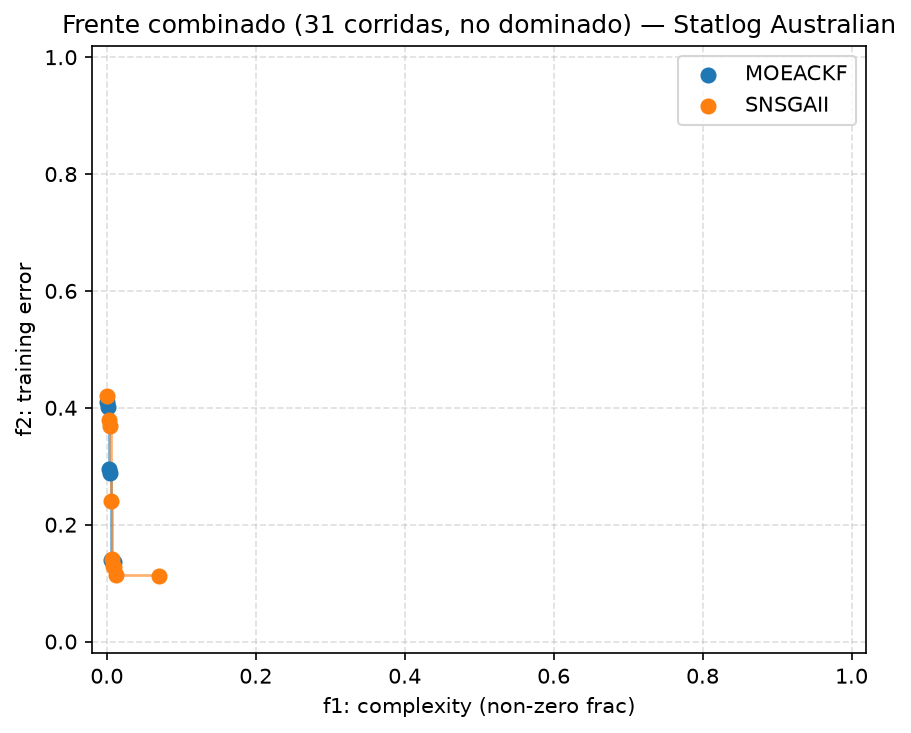
\includegraphics[width=0.75\textwidth]{fronts/ds1_combined_front.png}
\caption{Frente combinado (unión no dominada de las 31 corridas) de MOEACKF vs.\ SNSGAII,
dataset 1 (Statlog Australian).}
\label{fig:combined-front-ds1}
\end{figure}

Este resultado (Figura~\ref{fig:combined-front-ds1}) matiza el hallazgo de HV: pese a tener menos
puntos, el frente combinado de MOEACKF domina en mayor proporción al de SNSGAII que a la inversa.
Esto indica que la ventaja de SNSGAII en HV proviene de cubrir una región más amplia del espacio
de soluciones, y no de que cada punto individual de SNSGAII sea mejor que su contraparte de
MOEACKF.

\textbf{Error por banda de complejidad} (deciles sobre el pool de puntos crudos de ambos
algoritmos), Figura~\ref{fig:complexity-bands-ds1}.

\begin{figure}[htbp]
\centering
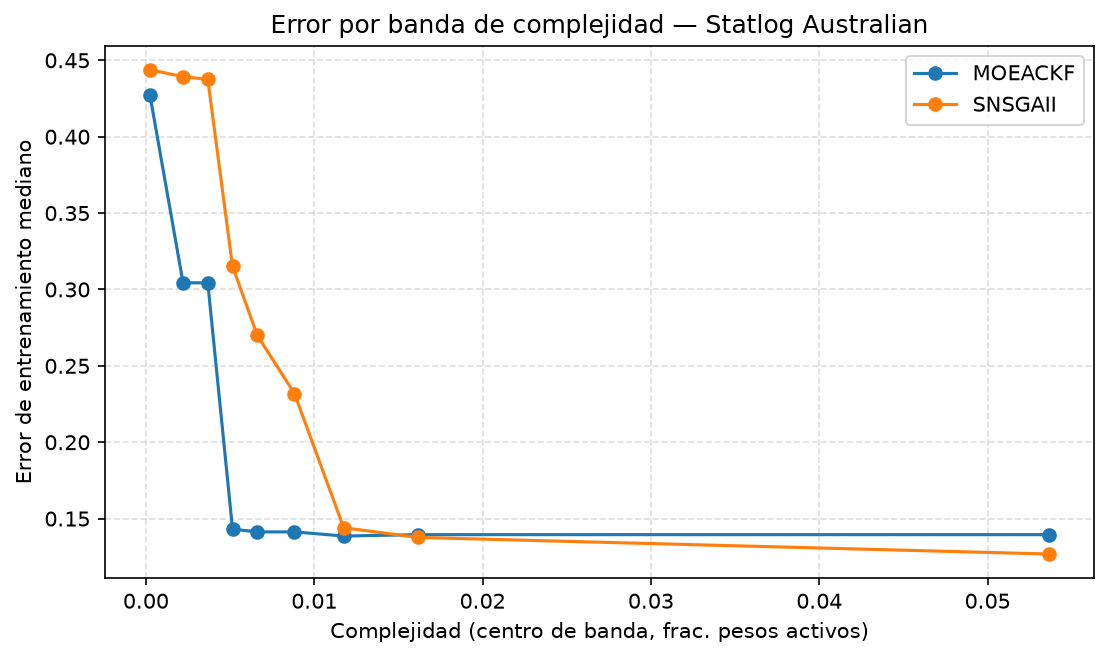
\includegraphics[width=0.75\textwidth]{fronts/ds1_complexity_bands.png}
\caption{Error de entrenamiento mediano por banda de complejidad, dataset 1 (Statlog
Australian).}
\label{fig:complexity-bands-ds1}
\end{figure}

MOEACKF domina claramente en las bandas de complejidad baja y media (hasta $\sim0.0132$), con
errores notablemente menores que SNSGAII en el mismo rango (p.\,ej.\ $0.143$ vs.\ $0.315$).
SNSGAII solo iguala y supera levemente a MOEACKF en la banda más alta, pero es justamente ahí
donde concentra la mayoría de sus puntos (37 de 189, frente a uno solo de MOEACKF). Esto indica
que el HV agregado de SNSGAII se explica por operar consistentemente en esa región de mayor
complejidad y precisión, y no por dominar en todo el espectro.

\subsubsection{Convergencia}
\label{sec:ds1-convergencia}

\begin{figure}[htbp]
\centering
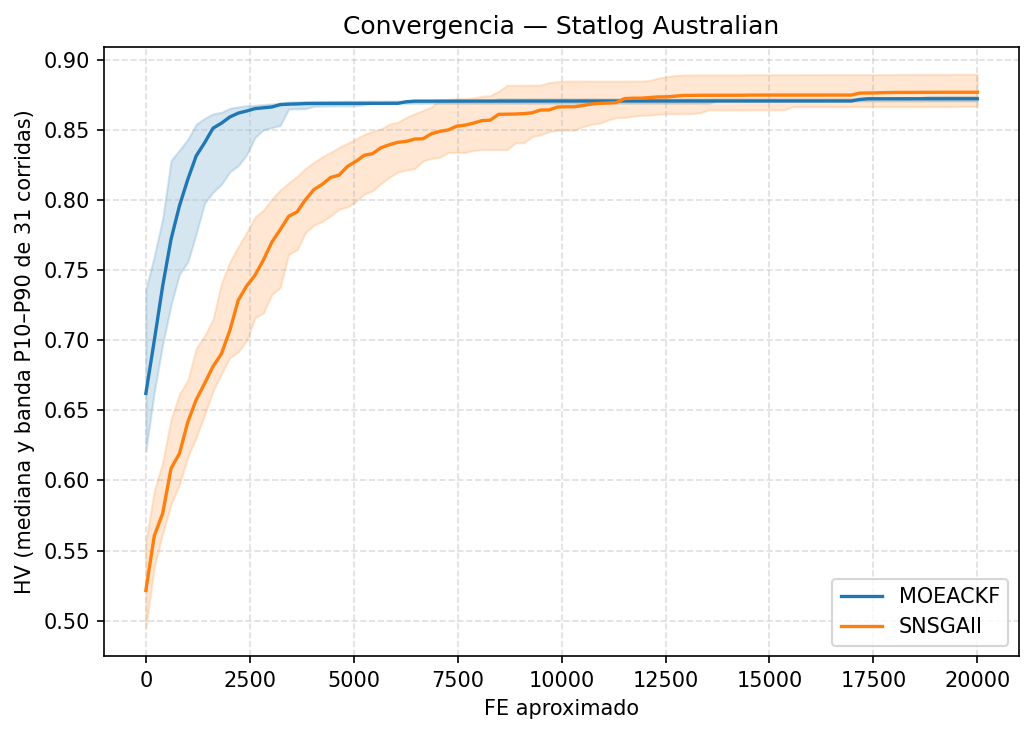
\includegraphics[width=0.75\textwidth]{convergence/ds1_convergence.png}
\caption{Curva de convergencia (HV mediano y banda P10--P90 de 31 corridas vs.\ FE aproximado),
dataset 1 (Statlog Australian).}
\label{fig:convergence-ds1}
\end{figure}

Según la Figura~\ref{fig:convergence-ds1}, MOEACKF converge mucho más rápido al comienzo: sube
abruptamente y se estabiliza ya cerca de $\text{FE}\approx3000$--$4000$ en
$\text{HV}\approx0.87$. SNSGAII, en cambio, arranca más bajo y asciende de forma más gradual,
y solo supera el plateau de MOEACKF alrededor de $\text{FE}\approx11000$--$13000$, para
terminar levemente más alto.

\textbf{Velocidad de convergencia} (FE hasta alcanzar el 95\% del HV final de cada corrida),
Tabla~\ref{tab:convergence-speed-ds1}.

\begin{table}[htbp]
\centering
\small
\caption{FE aproximado hasta alcanzar el 95\% del HV final de cada corrida, dataset 1.}
\label{tab:convergence-speed-ds1}
\begin{tabular}{@{}lccc@{}}
\toprule
\textbf{Grupo} & \textbf{Mediana [IQR]} & \textbf{$p$ (Wilcoxon)} &
  \Atwelve \\
\midrule
MOEACKF & $1212.1\ [969.7,\,1515.2]$ & --- & --- \\
SNSGAII & $5226.1\ [5025.1,\,6733.7]$ & $9.31\times10^{-10}$* & 0.000 \\
\bottomrule
\end{tabular}
\end{table}

La diferencia es significativa tras corrección ($p=4.66\times10^{-9}$), con $\Atwelve=0.000$: en
las 31 corridas, MOEACKF alcanza el 95\% de su propio HV final antes que SNSGAII, en promedio
$\sim4.3\times$ más rápido. Esto cuantifica lo que ya se observa en la curva: MOEACKF es
sistemáticamente más rápido para acercarse a su techo, pero ese techo resulta más bajo que el de
SNSGAII.

\subsubsection{Plataforma: SNN (C++) vs.\ ANN (MATLAB original)}
\label{sec:ds1-plataforma}

\begin{table}[htbp]
\centering
\small
\caption{MOEACKF: SNN vs.\ ANN (MATLAB), dataset 1.}
\label{tab:platform-moeackf-ds1}
\begin{tabular}{@{}lp{3.2cm}p{3.2cm}cc@{}}
\toprule
\textbf{Indicador} & \textbf{MOEACKF: SNN} & \textbf{MOEACKF: ANN-MATLAB} &
  \textbf{$p$ (Mann-Whitney)} & \Atwelve \\
\midrule
HV & mediana $0.8721\ [0.8704,\,0.8721]$ & mediana $0.8891\ [0.8891,\,0.8907]$ &
  $1.37\times10^{-11}$* & 0.000 \\
Complejidad & mediana $0.0088\ [0.0074,\,0.0140]$ & mediana $0.0203\ [0.0140,\,0.0390]$ &
  $2.58\times10^{-7}$* & 0.120 \\
Accuracy & mediana $0.8605\ [0.8587,\,0.8605]$ & mediana $0.8804\ [0.8804,\,0.8822]$ &
  $5.06\times10^{-12}$* & 0.000 \\
\bottomrule
\end{tabular}

\bigskip
\centering
\caption{SNSGAII: SNN vs.\ ANN (MATLAB), dataset 1.}
\label{tab:platform-snsgaii-ds1}
\begin{tabular}{@{}lp{3.2cm}p{3.2cm}cc@{}}
\toprule
\textbf{Indicador} & \textbf{SNSGAII: SNN} & \textbf{SNSGAII: ANN-MATLAB} &
  \textbf{$p$ (Mann-Whitney)} & \Atwelve \\
\midrule
HV & mediana $0.8767\ [0.8702,\,0.8856]$ & mediana $0.8972\ [0.8948,\,0.8979]$ &
  $5.89\times10^{-11}$* & 0.016 \\
Complejidad & mediana $0.0221\ [0.0132,\,0.0375]$ & mediana $0.0265\ [0.0265,\,0.1256]$ &
  $1.33\times10^{-4}$* & 0.221 \\
Accuracy & mediana $0.8678\ [0.8605,\,0.8768]$ & mediana $0.8895\ [0.8877,\,0.8904]$ &
  $3.12\times10^{-11}$* & 0.011 \\
\bottomrule
\end{tabular}
\end{table}

Las seis comparaciones (Tablas~\ref{tab:platform-moeackf-ds1} y \ref{tab:platform-snsgaii-ds1})
son significativas y se mantienen tras la corrección de Holm-Bonferroni (familia
\texttt{plataforma}, $p$ ajustados entre $1.52\times10^{-11}$ y $1.18\times10^{-10}$ para
HV/accuracy, y $2.58\times10^{-7}$/$1.33\times10^{-4}$ para complejidad). La implementación
original en ANN (MATLAB) supera de forma consistente a la SNN en HV y accuracy para ambos
algoritmos, con una brecha de accuracy de $\sim0.02$ en los dos casos, un patrón esperable si se
considera que la dinámica de disparo añade una capa de aproximación que una ANN estándar no
enfrenta. La red de mejor accuracy en ANN también tiende a ser más densa ($0.030$ vs.\ $0.011$
para MOEACKF); en el caso de SNSGAII la mediana es similar, pero la media y el rango se disparan
debido a algunas corridas en MATLAB que alcanzan redes casi densas.

\subsubsection{Bootstrap vs.\ evaluación completa}
\label{sec:ds1-bootstrap}

\begin{sidewaystable}
\centering
\small
\caption{HV con evaluación normal vs.\ bootstrap, y multiplicador de tiempo de cómputo, dataset 1.}
\label{tab:bootstrap-ds1}
\begin{tabular}{@{}lp{3.4cm}p{3.4cm}ccp{3.6cm}@{}}
\toprule
\textbf{Algoritmo} & \textbf{Normal} & \textbf{Bootstrap} & \textbf{$p$ (Wilcoxon)} & \Atwelve &
  \textbf{Tiempo mediano ($\times$)} \\
\midrule
MOEACKF & mediana $0.8721\ [0.8704,\,0.8721]$ & mediana $0.8830\ [0.8814,\,0.8854]$ &
  $9.31\times10^{-10}$* & 0.000 & $209\text{ s} \rightarrow 1734\text{ s}$ ($\times8.3$) \\
SNSGAII & mediana $0.8767\ [0.8702,\,0.8856]$ & mediana $0.8879\ [0.8829,\,0.8909]$ &
  $8.66\times10^{-5}$* & 0.258 & $940\text{ s} \rightarrow 14195\text{ s}$ ($\times15.1$) \\
\bottomrule
\end{tabular}
\end{sidewaystable}

Ambas diferencias (Tabla~\ref{tab:bootstrap-ds1}) son significativas tras corrección (familia
\texttt{bootstrap}, $p=1.86\times10^{-9}$ y $8.66\times10^{-5}$). El remuestreo bootstrap mejora
el HV de los dos algoritmos en este dataset: de forma casi absoluta en el caso de MOEACKF
($\Atwelve=0.000$, bootstrap gana las 31 corridas) y con un efecto igualmente grande en SNSGAII,
aunque a un costo computacional considerable ($8.3\times$ y $15.1\times$, respectivamente).

\subsubsection{Tiempo de cómputo}
\label{sec:ds1-tiempo}

\begin{table}[htbp]
\centering
\small
\caption{Tiempo de ejecución (\texttt{time\_s}), dataset 1, $N=15$ corridas pareadas
(\texttt{time\_experiments}).}
\label{tab:time-ds1}
\begin{tabular}{@{}lccc@{}}
\toprule
\textbf{Grupo} & \textbf{Mediana [IQR]} & \textbf{$p$ (Wilcoxon)} &
  \Atwelve \\
\midrule
MOEACKF & $285.6\ [263.7,\,288.2]$ s & --- & --- \\
SNSGAII & $259.6\ [258.4,\,260.5]$ s & $0.00153$* & 0.867 \\
\bottomrule
\end{tabular}
\end{table}

Según la Tabla~\ref{tab:time-ds1}, la diferencia es significativa (familia \texttt{tiempo},
$m=1$, sin corrección adicional): SNSGAII resulta más rápido, con un efecto grande
($\Atwelve=0.867$) y con mucha menos variabilidad entre corridas (DE$=2.5$s frente a $15.4$s de
MOEACKF).

\subsection{Dataset 2 --- Climate}
\label{sec:ds2}

\subsubsection{Hipervolumen (HV)}
\label{sec:ds2-hv}

\paragraph{Resultados}

\begin{table}[htbp]
\centering
\small
\caption{Hipervolumen (HV) de MOEACKF y SNSGAII en el dataset 2 (Climate), $N=31$ corridas
pareadas por seed.}
\label{tab:hv-ds2}
\begin{tabular}{@{}lcc@{}}
\toprule
\textbf{Algoritmo} & \textbf{N} & \textbf{Mediana [IQR]} \\
\midrule
MOEACKF & 31 & $0.9256\ [0.9255,\,0.9285]$ \\
SNSGAII & 31 & $0.9278\ [0.9257,\,0.9278]$ \\
\bottomrule
\end{tabular}
\end{table}

Los resultados descriptivos se resumen en la Tabla~\ref{tab:hv-ds2}. La prueba de Wilcoxon
signed-rank no encuentra una diferencia significativa entre ambos algoritmos ($W=199.0$,
$p=0.347$, $\alpha=0.05$), y esta falta de significancia se mantiene tras corrección
($p=0.694$). SNSGAII superó a MOEACKF en 23 de las 31 corridas (74.2\,\%), lo que corresponde a
$\Atwelve=0.258$.

\paragraph{Discusión}

Este dataset es el único caso en que el conteo de ``victorias'' por corrida ($\Atwelve$) y el
resultado de significancia del Wilcoxon \textbf{divergen}: SNSGAII gana más seguido, pero por
márgenes mínimos (diferencia mediana de solo $0.00016$), mientras que en las pocas corridas donde
gana MOEACKF lo hace por márgenes considerablemente mayores (su máximo, $0.9361$, supera
ampliamente el máximo de SNSGAII, $0.9299$). En conjunto, no hay evidencia suficiente de una
diferencia real entre ambos algoritmos en HV para este dataset, ya que ambos convergen a una
región muy similar y estrecha del espacio de soluciones. Las secciones siguientes muestran que,
aun sin diferencia en HV, los frentes de cada algoritmo llegan a esa región por caminos muy
distintos.

\subsubsection{Frentes de Pareto}
\label{sec:ds2-fronts}

\textbf{Solución de mejor accuracy por corrida}, Tabla~\ref{tab:fronts-ds2}.

\begin{table}[htbp]
\centering
\small
\caption{Indicadores de la solución de mejor accuracy por corrida, MOEACKF vs.\ SNSGAII,
dataset 2.}
\label{tab:fronts-ds2}
\begin{tabular}{@{}lp{3.5cm}p{3.5cm}cc@{}}
\toprule
\textbf{Indicador} & \textbf{MOEACKF} & \textbf{SNSGAII} & \textbf{$p$ (Wilcoxon)} & \Atwelve \\
\midrule
Complejidad (frac.\ pesos activos) &
  mediana $0.0190\ [0.0083,\,0.0363]$ &
  mediana $0.0036\ [0.0024,\,0.0036]$ &
  $9.31\times10^{-10}$* & 1.000 \\
Error de entrenamiento &
  mediana $0.0810\ [0.0775,\,0.0810]$ &
  mediana $0.0787\ [0.0787,\,0.0810]$ &
  $0.5345$ & 0.565 \\
Tamaño del frente &
  mediana $7\ [6,\,7]$ &
  mediana $3\ [3,\,4]$ &
  $1.42\times10^{-6}$* & 0.984 \\
\bottomrule
\end{tabular}
\end{table}

La complejidad y el tamaño del frente siguen siendo significativos tras corrección
($p=4.66\times10^{-9}$ y $5.69\times10^{-6}$), mientras que el error de la mejor red no lo es
($p=0.694$, igual que el HV agregado). El resultado más llamativo es el de complejidad: SNSGAII
encuentra una red de mejor accuracy \textbf{extremadamente rala} (mediana $0.0036$, apenas
$\sim3$ pesos activos de 840) con $\Atwelve=1.000$ (gana las 31 corridas), logrando un error
estadísticamente indistinguible del de MOEACKF. Este último necesita, en cambio, una red bastante
más densa y variable (mediana $0.019$, con corridas que llegan mucho más alto: DE$=0.14$, casi el
doble de la propia mediana). SNSGAII también retiene un frente considerablemente más pequeño
(mediana 3 vs.\ 7).

\textbf{Frente combinado y C-metric}: tamaño MOEACKF$=8$, SNSGAII$=4$.
$C(\text{MOEACKF},\text{SNSGAII})=0.500$, $C(\text{SNSGAII},\text{MOEACKF})=0.500$ --- cobertura
perfectamente simétrica pese a la diferencia de tamaño (Figura~\ref{fig:combined-front-ds2}).

\begin{figure}[htbp]
\centering
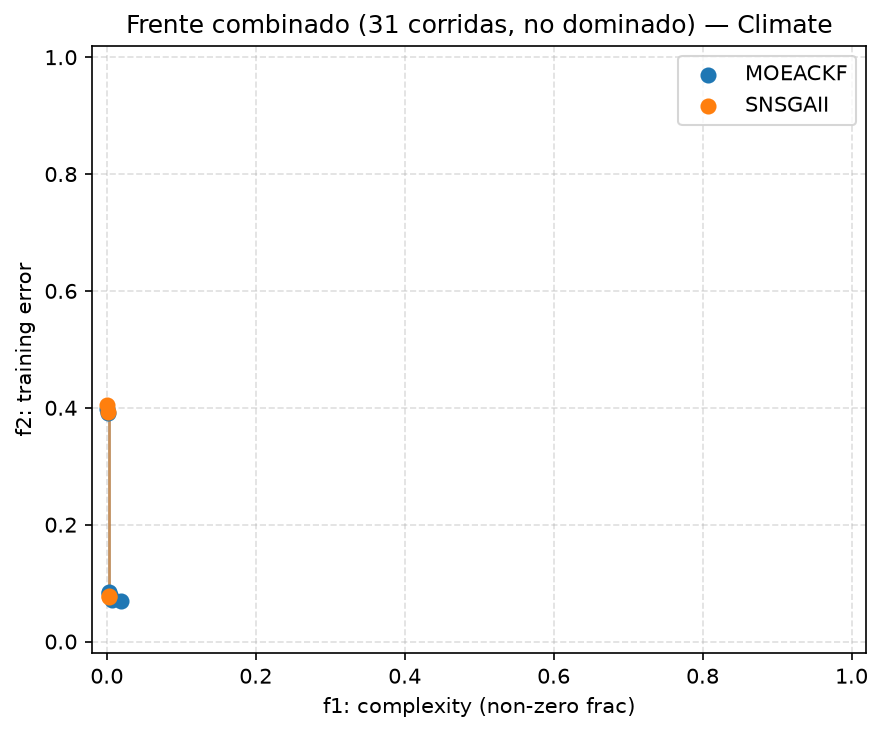
\includegraphics[width=0.75\textwidth]{fronts/ds2_combined_front.png}
\caption{Frente combinado de MOEACKF vs.\ SNSGAII, dataset 2 (Climate).}
\label{fig:combined-front-ds2}
\end{figure}

\textbf{Error por banda de complejidad}, Figura~\ref{fig:complexity-bands-ds2}.

\begin{figure}[htbp]
\centering
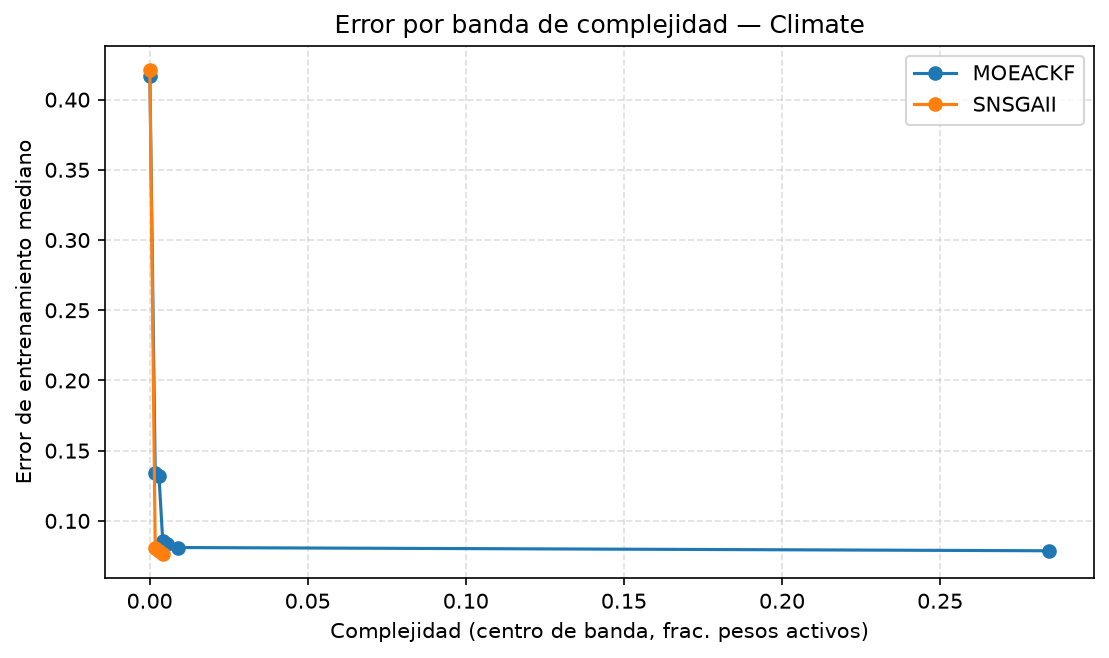
\includegraphics[width=0.75\textwidth]{fronts/ds2_complexity_bands.png}
\caption{Error de entrenamiento mediano por banda de complejidad, dataset 2 (Climate).}
\label{fig:complexity-bands-ds2}
\end{figure}

SNSGAII prácticamente no tiene puntos más allá de la banda de complejidad $0.0036$--$0.0048$: sus
31 corridas concentran casi toda su masa en las bandas de menor complejidad, donde su error es
consistentemente \textbf{menor} que el de MOEACKF en las mismas bandas ($0.081$ vs.\ $0.134$).
Climate parece ser, entonces, un dataset donde SNSGAII se especializa en soluciones ultra-ralas y
lo hace con buenos resultados, mientras que MOEACKF explora más sin obtener una ganancia
proporcional, lo cual es coherente con que el HV agregado no distinga a los algoritmos
(\S\ref{sec:ds2-hv}).

\subsubsection{Convergencia}
\label{sec:ds2-convergencia}

\begin{figure}[htbp]
\centering
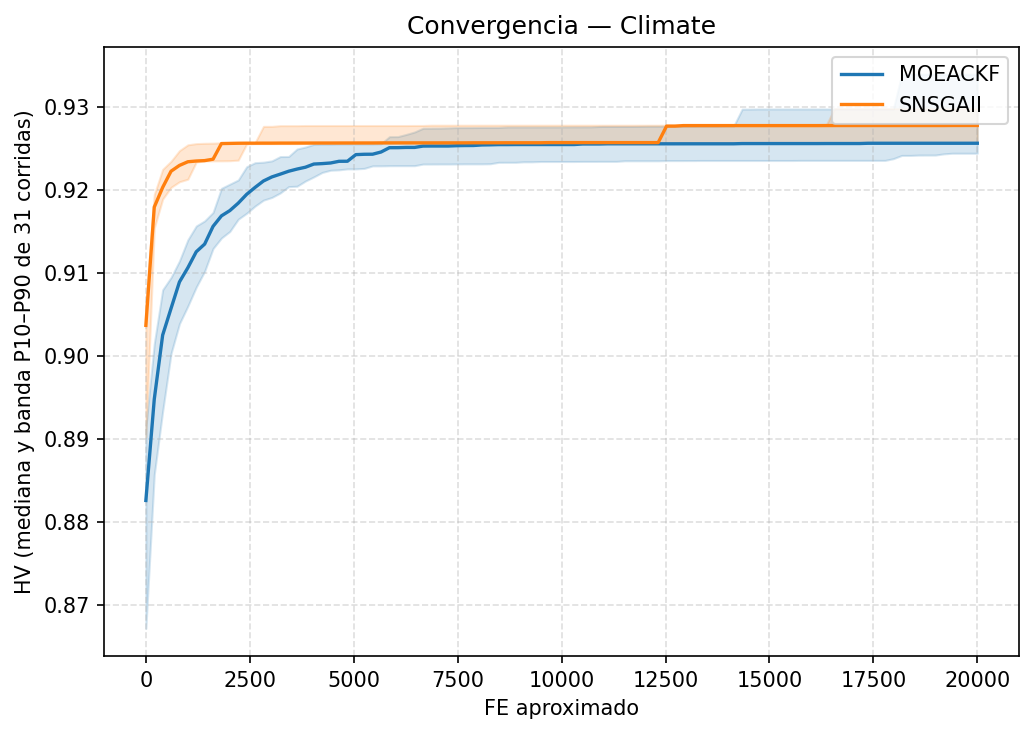
\includegraphics[width=0.75\textwidth]{convergence/ds2_convergence.png}
\caption{Curva de convergencia, dataset 2 (Climate).}
\label{fig:convergence-ds2}
\end{figure}

\textbf{Velocidad de convergencia} (FE hasta 95\% y 90\% del HV final), Tabla~\ref{tab:convergence-speed-ds2}.

\begin{table}[htbp]
\centering
\small
\caption{FE aproximado hasta alcanzar el 95\% y el 90\% del HV final de cada corrida, dataset 2.}
\label{tab:convergence-speed-ds2}
\begin{tabular}{@{}lp{3.6cm}p{3.6cm}cc@{}}
\toprule
\textbf{Umbral} & \textbf{MOEACKF} & \textbf{SNSGAII} & \textbf{$p$ (Wilcoxon)} & \Atwelve \\
\midrule
95\% del HV final &
  mediana $0\ [0,\,127.4]$ &
  mediana $0\ [0,\,0]$ &
  $4.75\times10^{-4}$* & 0.694 \\
90\% del HV final &
  mediana $0\ [0,\,0]$ &
  mediana $0\ [0,\,0]$ &
  $1.0$ (sin diferencia) & 0.500 \\
\bottomrule
\end{tabular}
\end{table}

Climate constituye un caso límite: en las 31 corridas de \textbf{ambos} algoritmos, la población
inicial (generación 0) ya alcanza el 90\% del HV final, por lo que no hay evidencia de diferencia
alguna en ese umbral ($x_i=y_i$ en los 31 pares). Al 95\% sí aparece una diferencia significativa
(tras corrección, $p=1.43\times10^{-3}$), con SNSGAII llegando más seguido ya en
$\text{FE}\approx0$. Esto confirma cuantitativamente lo que sugiere la curva
(Figura~\ref{fig:convergence-ds2}): Climate es un problema comparativamente ``saturado'', en el
que el margen de mejora sobre la población inicial es pequeño para ambos algoritmos, de modo que
la ``velocidad de convergencia'' aquí mide más bien qué tan rápido se estabiliza la búsqueda que
una carrera real de optimización.

\subsubsection{Plataforma: SNN (C++) vs.\ ANN (MATLAB original)}
\label{sec:ds2-plataforma}

\begin{table}[htbp]
\centering
\small
\caption{MOEACKF: SNN vs.\ ANN (MATLAB), dataset 2.}
\label{tab:platform-moeackf-ds2}
\begin{tabular}{@{}lp{3.2cm}p{3.2cm}cc@{}}
\toprule
\textbf{Indicador} & \textbf{MOEACKF: SNN} & \textbf{MOEACKF: ANN-MATLAB} &
  \textbf{$p$ (Mann-Whitney)} & \Atwelve \\
\midrule
HV & mediana $0.9256\ [0.9255,\,0.9285]$ & mediana $0.9767\ [0.9747,\,0.9770]$ &
  $1.40\times10^{-11}$* & 0.000 \\
Complejidad & mediana $0.0190\ [0.0083,\,0.0363]$ & mediana $0.0487\ [0.0399,\,0.0662]$ &
  $2.37\times10^{-4}$* & 0.228 \\
Accuracy & mediana $0.9190\ [0.9190,\,0.9225]$ & mediana $0.9768\ [0.9745,\,0.9768]$ &
  $6.06\times10^{-12}$* & 0.000 \\
\bottomrule
\end{tabular}

\bigskip
\centering
\caption{SNSGAII: SNN vs.\ ANN (MATLAB), dataset 2.}
\label{tab:platform-snsgaii-ds2}
\begin{tabular}{@{}lp{3.2cm}p{3.2cm}cc@{}}
\toprule
\textbf{Indicador} & \textbf{SNSGAII: SNN} & \textbf{SNSGAII: ANN-MATLAB} &
  \textbf{$p$ (Mann-Whitney)} & \Atwelve \\
\midrule
HV & mediana $0.9278\ [0.9257,\,0.9278]$ & mediana $0.9477\ [0.9440,\,0.9539]$ &
  $1.39\times10^{-11}$* & 0.000 \\
Complejidad & mediana $0.0036\ [0.0024,\,0.0036]$ & mediana $0.9114\ [0.7316,\,0.9601]$ &
  $7.72\times10^{-12}$* & 0.000 \\
Accuracy & mediana $0.9213\ [0.9190,\,0.9213]$ & mediana $0.9653\ [0.9630,\,0.9699]$ &
  $8.20\times10^{-12}$* & 0.000 \\
\bottomrule
\end{tabular}
\end{table}

Todas las comparaciones son significativas tras corrección (Tablas~\ref{tab:platform-moeackf-ds2}
y \ref{tab:platform-snsgaii-ds2}). La brecha ANN-SNN en HV es la más grande de los cuatro
datasets para MOEACKF ($0.976$ vs.\ $0.928$, $\sim5$ puntos). La complejidad, en cambio, diverge
fuertemente según el algoritmo: para MOEACKF la red ANN es apenas algo más rala que la SNN
($0.056$ vs.\ $0.075$), mientras que para SNSGAII la red ANN de mejor accuracy es \textbf{casi
completamente densa} (mediana $0.911$, más del 90\% de los pesos activos) frente a la red SNN
ultra-rala descrita en \S\ref{sec:ds2-fronts} (mediana $0.0036$). Se trata de la divergencia de
plataforma más extrema del estudio: para llegar a su mejor accuracy, SNSGAII-ANN necesita casi
todos los pesos activos, mientras que SNSGAII-SNN logra un error estadísticamente similar
(\S\ref{sec:ds2-fronts}) con una fracción minúscula de la red. Sujeto a las salvedades señaladas
en \S\ref{sec:limitaciones} (RNG e implementación distintos entre plataformas), esto sugiere que
el sustrato spiking podría favorecer soluciones ralas para esta combinación de algoritmo y
dataset en particular, una hipótesis a confirmar y no una conclusión causal con el diseño
actual.

\subsubsection{Bootstrap vs.\ evaluación completa}
\label{sec:ds2-bootstrap}

\begin{sidewaystable}
\centering
\small
\caption{HV con evaluación normal vs.\ bootstrap, y multiplicador de tiempo de cómputo, dataset 2.}
\label{tab:bootstrap-ds2}
\begin{tabular}{@{}lp{3.4cm}p{3.4cm}ccp{3.6cm}@{}}
\toprule
\textbf{Algoritmo} & \textbf{Normal} & \textbf{Bootstrap} & \textbf{$p$ (Wilcoxon)} & \Atwelve &
  \textbf{Tiempo mediano ($\times$)} \\
\midrule
MOEACKF & mediana $0.9256\ [0.9255,\,0.9285]$ & mediana $0.9401\ [0.9393,\,0.9415]$ &
  $9.31\times10^{-10}$* & 0.000 & $1805\text{ s} \rightarrow 8749\text{ s}$ ($\times4.8$) \\
SNSGAII & mediana $0.9278\ [0.9257,\,0.9278]$ & mediana $0.9399\ [0.9390,\,0.9408]$ &
  $9.31\times10^{-10}$* & 0.000 & $202\text{ s} \rightarrow 998\text{ s}$ ($\times4.9$) \\
\bottomrule
\end{tabular}
\end{sidewaystable}

Ambas diferencias (Tabla~\ref{tab:bootstrap-ds2}) son significativas tras corrección
($p=1.86\times10^{-9}$ en ambos casos). A diferencia del HV entre algoritmos, que no muestra
diferencia en este dataset (\S\ref{sec:ds2-hv}), el bootstrap sí produce una mejora grande y
perfectamente consistente ($\Atwelve=0.000$ en los dos algoritmos: bootstrap gana las 31
corridas), además con el menor costo relativo de tiempo de los cuatro datasets ($\times4.8$--$4.9$,
frente a $\times5$--$15$ en el resto).

\subsubsection{Tiempo de cómputo}
\label{sec:ds2-tiempo}

\begin{table}[htbp]
\centering
\small
\caption{Tiempo de ejecución (\texttt{time\_s}), dataset 2, $N=15$ corridas pareadas.}
\label{tab:time-ds2}
\begin{tabular}{@{}lccc@{}}
\toprule
\textbf{Grupo} & \textbf{Mediana [IQR]} & \textbf{$p$ (Wilcoxon)} &
  \Atwelve \\
\midrule
MOEACKF & $230.5\ [224.0,\,235.2]$ s & --- & --- \\
SNSGAII & $216.7\ [216.0,\,217.0]$ s & $8.54\times10^{-4}$* & 0.867 \\
\bottomrule
\end{tabular}
\end{table}

Según la Tabla~\ref{tab:time-ds2}, la diferencia vuelve a ser significativa: SNSGAII es más
rápido, con un efecto grande y con mucha menor variabilidad entre corridas.

\subsection{Dataset 3 --- German}
\label{sec:ds3}

\subsubsection{Hipervolumen (HV)}
\label{sec:ds3-hv}

\paragraph{Resultados}

\begin{table}[htbp]
\centering
\small
\caption{Hipervolumen (HV) de MOEACKF y SNSGAII en el dataset 3 (German), $N=31$ corridas
pareadas por seed.}
\label{tab:hv-ds3}
\begin{tabular}{@{}lcc@{}}
\toprule
\textbf{Algoritmo} & \textbf{N} & \textbf{Mediana [IQR]} \\
\midrule
MOEACKF & 31 & $0.7520\ [0.7452,\,0.7560]$ \\
SNSGAII & 31 & $0.7643\ [0.7547,\,0.7754]$ \\
\bottomrule
\end{tabular}
\end{table}

Los resultados descriptivos se resumen en la Tabla~\ref{tab:hv-ds3}. La prueba de Wilcoxon
signed-rank arroja una diferencia altamente significativa entre ambos algoritmos ($W=50.0$,
$p=2.8\times10^{-5}$), que se mantiene tras corrección ($p=8.47\times10^{-5}$). SNSGAII superó a
MOEACKF en 24 de las 31 corridas (77.4\,\%), lo que corresponde a $\Atwelve=0.226$ y a un efecto
\textbf{grande} a favor de SNSGAII.

\paragraph{Discusión}

Este es un resultado contundente a favor de SNSGAII: la diferencia de medianas ($0.0133$) y de
medias ($0.0134$) es la segunda mayor de los cuatro datasets y, a diferencia del dataset 2, aquí
la dirección del conteo de victorias y la magnitud de las diferencias coinciden. SNSGAII vuelve a
mostrar mayor dispersión que MOEACKF (DE$=0.0160$ vs.\ $0.0060$), pero incluso su corrida más
baja ($0.7349$) queda cerca de la mediana de MOEACKF, de modo que la mayor variabilidad no
compromete de forma importante la fiabilidad del resultado.

\subsubsection{Frentes de Pareto}
\label{sec:ds3-fronts}

\textbf{Solución de mejor accuracy por corrida}, Tabla~\ref{tab:fronts-ds3}.

\begin{table}[htbp]
\centering
\small
\caption{Indicadores de la solución de mejor accuracy por corrida, MOEACKF vs.\ SNSGAII,
dataset 3.}
\label{tab:fronts-ds3}
\begin{tabular}{@{}lp{3.5cm}p{3.5cm}cc@{}}
\toprule
\textbf{Indicador} & \textbf{MOEACKF} & \textbf{SNSGAII} & \textbf{$p$ (Wilcoxon)} & \Atwelve \\
\midrule
Complejidad (frac.\ pesos activos) &
  mediana $0.0065\ [0.0042,\,0.0269]$ &
  mediana $0.0296\ [0.0204,\,0.0468]$ &
  $0.00915$* & 0.226 \\
Error de entrenamiento &
  mediana $0.2725\ [0.2681,\,0.2800]$ &
  mediana $0.2587\ [0.2462,\,0.2694]$ &
  $8.90\times10^{-5}$* & 0.790 \\
Tamaño del frente &
  mediana $5\ [4,\,7]$ &
  mediana $9\ [8,\,10.5]$ &
  $1.85\times10^{-5}$* & 0.161 \\
\bottomrule
\end{tabular}
\end{table}

Los tres indicadores resultan significativos tras corrección ($p=9.15\times10^{-3}$,
$1.78\times10^{-4}$, $7.41\times10^{-5}$), reproduciendo el mismo patrón cualitativo observado en
el dataset 1: SNSGAII incurre en más complejidad en su mejor red ($0.030$ vs.\ $0.007$) a cambio
de un menor error ($0.259$ vs.\ $0.273$, efecto grande) y retiene un frente sustancialmente más
grande (9 vs.\ 5). De los cuatro datasets, este es el más consistente con la idea de que SNSGAII
gana explorando redes más densas y numerosas.

\textbf{Frente combinado y C-metric}: tamaño MOEACKF$=6$, SNSGAII$=13$.
$C(\text{MOEACKF},\text{SNSGAII})=0.308$, $C(\text{SNSGAII},\text{MOEACKF})=0.333$ --- cobertura
mutua similar pese a que el frente de SNSGAII es más del doble de grande
(Figura~\ref{fig:combined-front-ds3}).

\begin{figure}[htbp]
\centering
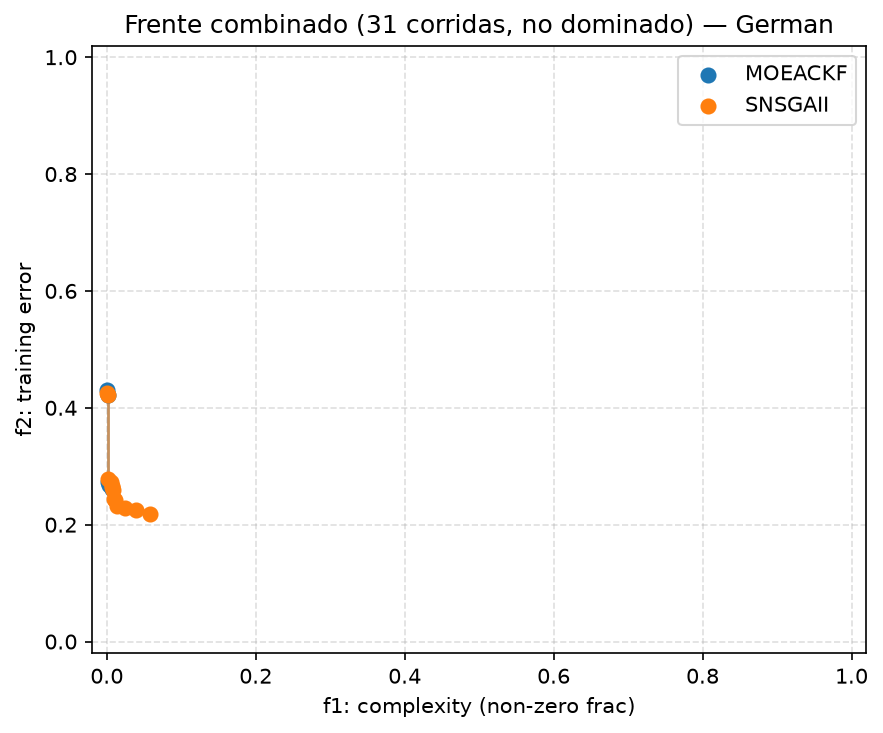
\includegraphics[width=0.75\textwidth]{fronts/ds3_combined_front.png}
\caption{Frente combinado de MOEACKF vs.\ SNSGAII, dataset 3 (German).}
\label{fig:combined-front-ds3}
\end{figure}

\textbf{Error por banda de complejidad}, Figura~\ref{fig:complexity-bands-ds3}.

\begin{figure}[htbp]
\centering
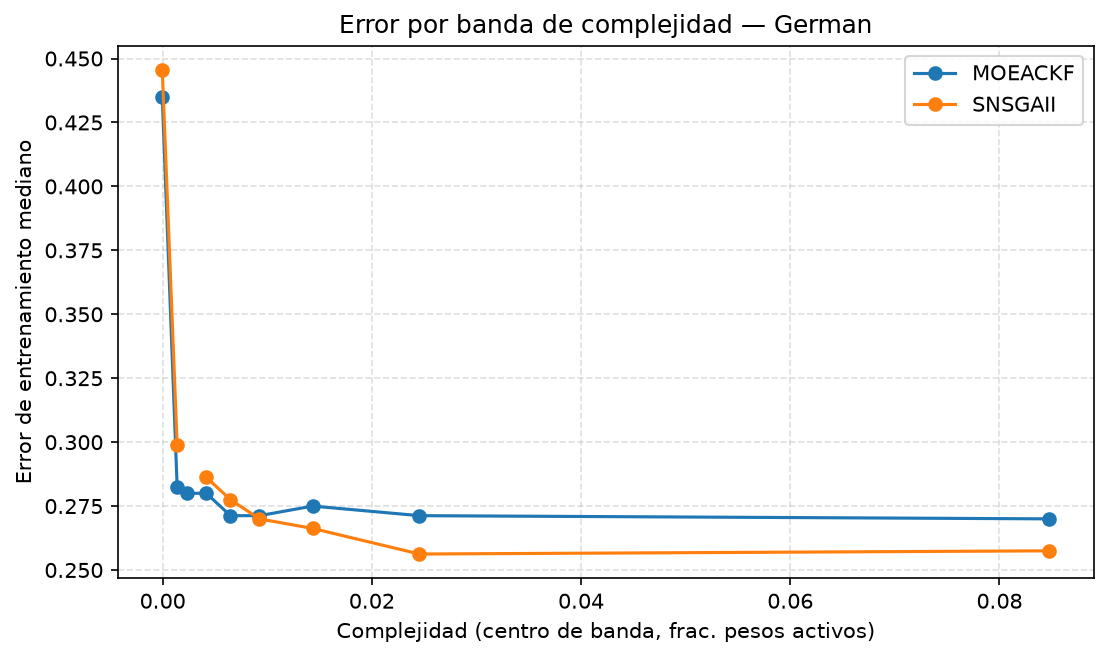
\includegraphics[width=0.75\textwidth]{fronts/ds3_complexity_bands.png}
\caption{Error de entrenamiento mediano por banda de complejidad, dataset 3 (German).}
\label{fig:complexity-bands-ds3}
\end{figure}

En las bandas de menor complejidad ambos algoritmos se comportan de forma similar, con MOEACKF
incluso algo mejor; sin embargo, a partir de complejidad $\geq0.0056$ SNSGAII pasa a tener un
error consistentemente menor, y la brecha se ensancha hacia las bandas más altas ($0.256$ vs.\
$0.271$). Esto indica que SNSGAII aprovecha mejor la complejidad adicional en este dataset, lo
cual es coherente con su frente combinado más grande (13 vs.\ 6 puntos) y con la ventaja de HV
descrita en \S\ref{sec:ds3-hv}.

\subsubsection{Convergencia}
\label{sec:ds3-convergencia}

\begin{figure}[htbp]
\centering
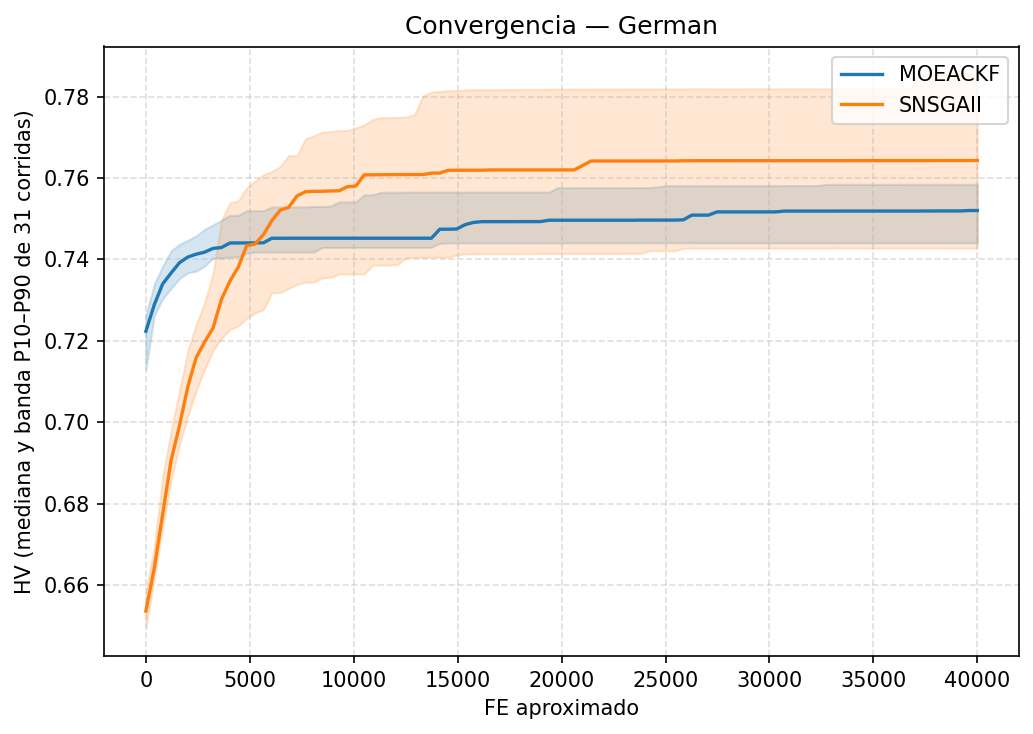
\includegraphics[width=0.75\textwidth]{convergence/ds3_convergence.png}
\caption{Curva de convergencia, dataset 3 (German).}
\label{fig:convergence-ds3}
\end{figure}

La curva (Figura~\ref{fig:convergence-ds3}) muestra a SNSGAII arrancando mucho más bajo
($\sim0.654$) y ascendiendo con pendiente pronunciada, hasta cruzar a MOEACKF alrededor de
$\text{FE}\approx4500$--$5000$ y terminar por encima de él ($\sim0.764$ vs.\ $\sim0.752$),
mientras que MOEACKF se aplana muy temprano.

\textbf{Velocidad de convergencia} (FE hasta 95\% del HV final), Tabla~\ref{tab:convergence-speed-ds3}.

\begin{table}[htbp]
\centering
\small
\caption{FE aproximado hasta alcanzar el 95\% del HV final de cada corrida, dataset 3.}
\label{tab:convergence-speed-ds3}
\begin{tabular}{@{}lccc@{}}
\toprule
\textbf{Grupo} & \textbf{Mediana [IQR]} & \textbf{$p$ (Wilcoxon)} &
  \Atwelve \\
\midrule
MOEACKF & $0\ [0,\,0]$ & --- & --- \\
SNSGAII & $3408.5\ [2456.1,\,3909.8]$ & $9.31\times10^{-10}$* & 0.000 \\
\bottomrule
\end{tabular}
\end{table}

La diferencia es significativa tras corrección ($p=4.66\times10^{-9}$), y arroja un resultado
aparentemente paradójico, aunque coherente con la curva: si bien SNSGAII logra el HV
\textbf{final} más alto (\S\ref{sec:ds3-hv}), es MOEACKF quien llega casi instantáneamente
(mediana $\text{FE}\approx0$) al 95\% de su propio techo, más bajo, pero alcanzado de inmediato,
mientras que SNSGAII necesita $\sim3400$ FE (8.5\% del presupuesto total de 40000) para llegar al
95\% de un techo más alto. Es un ejemplo claro del trade-off entre velocidad y calidad: MOEACKF
se estabiliza rápido en un techo menor, mientras que SNSGAII tarda más en llegar a uno mayor.

\subsubsection{Plataforma: SNN (C++) vs.\ ANN (MATLAB original)}
\label{sec:ds3-plataforma}

\begin{table}[htbp]
\centering
\small
\caption{MOEACKF: SNN vs.\ ANN (MATLAB), dataset 3.}
\label{tab:platform-moeackf-ds3}
\begin{tabular}{@{}lp{3.2cm}p{3.2cm}cc@{}}
\toprule
\textbf{Indicador} & \textbf{MOEACKF: SNN} & \textbf{MOEACKF: ANN-MATLAB} &
  \textbf{$p$ (Mann-Whitney)} & \Atwelve \\
\midrule
HV & mediana $0.7520\ [0.7452,\,0.7560]$ & mediana $0.8098\ [0.8082,\,0.8111]$ &
  $1.40\times10^{-11}$* & 0.000 \\
Complejidad & mediana $0.0065\ [0.0042,\,0.0269]$ & mediana $0.0413\ [0.0375,\,0.0644]$ &
  $1.26\times10^{-6}$* & 0.142 \\
Accuracy & mediana $0.7275\ [0.7200,\,0.7319]$ & mediana $0.7925\ [0.7906,\,0.7937]$ &
  $1.20\times10^{-11}$* & 0.000 \\
\bottomrule
\end{tabular}

\bigskip
\centering
\caption{SNSGAII: SNN vs.\ ANN (MATLAB), dataset 3.}
\label{tab:platform-snsgaii-ds3}
\begin{tabular}{@{}lp{3.2cm}p{3.2cm}cc@{}}
\toprule
\textbf{Indicador} & \textbf{SNSGAII: SNN} & \textbf{SNSGAII: ANN-MATLAB} &
  \textbf{$p$ (Mann-Whitney)} & \Atwelve \\
\midrule
HV & mediana $0.7643\ [0.7547,\,0.7754]$ & mediana $0.8119\ [0.8098,\,0.8132]$ &
  $1.40\times10^{-11}$* & 0.000 \\
Complejidad & mediana $0.0296\ [0.0204,\,0.0468]$ & mediana $0.8751\ [0.3506,\,0.9942]$ &
  $6.89\times10^{-10}$* & 0.044 \\
Accuracy & mediana $0.7412\ [0.7306,\,0.7538]$ & mediana $0.7975\ [0.7963,\,0.8006]$ &
  $1.33\times10^{-11}$* & 0.000 \\
\bottomrule
\end{tabular}
\end{table}

Todas las comparaciones son significativas tras corrección (Tablas~\ref{tab:platform-moeackf-ds3}
y \ref{tab:platform-snsgaii-ds3}), reproduciendo el mismo patrón observado en el dataset 2: la
red ANN de MOEACKF es moderadamente más densa que la SNN ($0.051$ vs.\ $0.018$), mientras que la
red ANN de SNSGAII vuelve a ser casi totalmente densa (mediana $0.875$) frente a una SNN mucho
más rala ($0.030$). La brecha de complejidad entre ANN y SNN para SNSGAII es sistemáticamente
mucho mayor que la de MOEACKF en los cuatro datasets (ver síntesis, \S\ref{sec:sintesis}), lo que
confirma que se trata de un patrón recurrente y no de un caso aislado de Climate.

\subsubsection{Bootstrap vs.\ evaluación completa}
\label{sec:ds3-bootstrap}

\begin{sidewaystable}
\centering
\small
\caption{HV con evaluación normal vs.\ bootstrap, y multiplicador de tiempo de cómputo, dataset 3.}
\label{tab:bootstrap-ds3}
\begin{tabular}{@{}lp{3.4cm}p{3.4cm}ccp{3.6cm}@{}}
\toprule
\textbf{Algoritmo} & \textbf{Normal} & \textbf{Bootstrap} & \textbf{$p$ (Wilcoxon)} & \Atwelve &
  \textbf{Tiempo mediano ($\times$)} \\
\midrule
MOEACKF & mediana $0.7520\ [0.7452,\,0.7560]$ & mediana $0.7567\ [0.7551,\,0.7588]$ &
  $1.95\times10^{-4}$* & 0.226 & $1207\text{ s} \rightarrow 6222\text{ s}$ ($\times5.2$) \\
SNSGAII & mediana $0.7643\ [0.7547,\,0.7754]$ & mediana $0.7549\ [0.7540,\,0.7568]$ &
  $0.0664$ & 0.710 & $914\text{ s} \rightarrow 6854\text{ s}$ ($\times7.5$) \\
\bottomrule
\end{tabular}
\end{sidewaystable}

Según la Tabla~\ref{tab:bootstrap-ds3}, MOEACKF mejora significativamente con bootstrap (tras
corrección, $p=3.91\times10^{-4}$), pero SNSGAII \textbf{no} lo hace ($p=0.066$, ni siquiera
sobrevive al umbral crudo de $0.05$): German es el primer dataset donde el bootstrap no ayuda de
forma uniforme a ambos algoritmos. Más aún, la dirección de $\Atwelve=0.710$ para SNSGAII sugiere
que la evaluación normal iguala o supera a la bootstrap más seguido que a la inversa, aunque sin
significancia estadística. No puede afirmarse, entonces, que el bootstrap perjudique a SNSGAII en
este dataset, pero tampoco que lo beneficie, pese a un costo de tiempo considerable
($\times7.5$).

\subsubsection{Tiempo de cómputo}
\label{sec:ds3-tiempo}

\begin{table}[htbp]
\centering
\small
\caption{Tiempo de ejecución (\texttt{time\_s}), dataset 3, $N=15$ corridas pareadas.}
\label{tab:time-ds3}
\begin{tabular}{@{}lccc@{}}
\toprule
\textbf{Grupo} & \textbf{Mediana [IQR]} & \textbf{$p$ (Wilcoxon)} &
  \Atwelve \\
\midrule
MOEACKF & $936.6\ [895.7,\,956.1]$ s & --- & --- \\
SNSGAII & $871.3\ [858.9,\,883.0]$ s & $4.27\times10^{-4}$* & 0.933 \\
\bottomrule
\end{tabular}
\end{table}

Según la Tabla~\ref{tab:time-ds3}, la diferencia es significativa: SNSGAII vuelve a ser más
rápido, con un efecto grande.

\subsection{Dataset 4 --- Sonar}
\label{sec:ds4}

\subsubsection{Hipervolumen (HV)}
\label{sec:ds4-hv}

\paragraph{Resultados}

\begin{table}[htbp]
\centering
\small
\caption{Hipervolumen (HV) de MOEACKF y SNSGAII en el dataset 4 (Sonar), $N=31$ corridas
pareadas por seed.}
\label{tab:hv-ds4}
\begin{tabular}{@{}lcc@{}}
\toprule
\textbf{Algoritmo} & \textbf{N} & \textbf{Mediana [IQR]} \\
\midrule
MOEACKF & 31 & $0.8274\ [0.8141,\,0.8432]$ \\
SNSGAII & 31 & $0.7812\ [0.7601,\,0.8059]$ \\
\bottomrule
\end{tabular}
\end{table}

Los resultados descriptivos se resumen en la Tabla~\ref{tab:hv-ds4}. La prueba de Wilcoxon
signed-rank arroja una diferencia altamente significativa entre ambos algoritmos ($W=60.0$,
$p=8.7\times10^{-5}$), que se mantiene tras corrección ($p=2.60\times10^{-4}$). MOEACKF superó a
SNSGAII en 22 de las 31 corridas (71.0\,\%), lo que corresponde a $\Atwelve=0.710$ y a un efecto
\textbf{grande} a favor de MOEACKF.

\paragraph{Discusión}

Sonar es el único dataset donde se invierte el patrón observado en los tres anteriores: MOEACKF
supera a SNSGAII de forma significativa y con la mayor diferencia absoluta de HV observada en
todo el estudio ($\Delta\text{media}=0.0417$). Es, además, el dataset con mayor varianza para
ambos algoritmos (DE$\approx0.03$--$0.04$), lo cual es consistente con que Sonar es, de los
cuatro, el de mayor dimensionalidad (60 features) y por lo tanto el de paisaje de optimización
más difícil. Las secciones siguientes muestran que aquí MOEACKF no gana solo en el agregado,
sino que domina en casi todos los indicadores individuales.

\subsubsection{Frentes de Pareto}
\label{sec:ds4-fronts}

\textbf{Solución de mejor accuracy por corrida}, Tabla~\ref{tab:fronts-ds4}.

\begin{table}[htbp]
\centering
\small
\caption{Indicadores de la solución de mejor accuracy por corrida, MOEACKF vs.\ SNSGAII,
dataset 4.}
\label{tab:fronts-ds4}
\begin{tabular}{@{}lp{3.5cm}p{3.5cm}cc@{}}
\toprule
\textbf{Indicador} & \textbf{MOEACKF} & \textbf{SNSGAII} & \textbf{$p$ (Wilcoxon)} & \Atwelve \\
\midrule
Complejidad (frac.\ pesos activos) &
  mediana $0.0429\ [0.0208,\,0.0847]$ &
  mediana $0.0159\ [0.0077,\,0.0270]$ &
  $1.07\times10^{-4}$* & 0.742 \\
Error de entrenamiento &
  mediana $0.1796\ [0.1677,\,0.1976]$ &
  mediana $0.2395\ [0.2126,\,0.2635]$ &
  $4.77\times10^{-5}$* & 0.194 \\
Tamaño del frente &
  mediana $12\ [9,\,13]$ &
  mediana $8\ [7,\,10.5]$ &
  $0.0166$* & 0.645 \\
\bottomrule
\end{tabular}
\end{table}

Los tres indicadores resultan significativos tras corrección ($p=2.60\times10^{-4}$,
$1.91\times10^{-4}$, $0.0166$). A diferencia de los datasets 1 y 3, aquí MOEACKF \textbf{no} cede
complejidad a cambio de precisión: su red de mejor accuracy es a la vez más densa ($0.043$ vs.\
$0.016$) y más precisa (error $0.180$ vs.\ $0.240$) que la de SNSGAII, y además retiene un frente
más grande (12 vs.\ 8). Es el único dataset donde un algoritmo domina de forma tan directa en los
tres indicadores del frente a la vez.

\textbf{Frente combinado y C-metric}: tamaño MOEACKF$=14$, SNSGAII$=14$ (iguales).
$C(\text{MOEACKF},\text{SNSGAII})=\mathbf{0.857}$, $C(\text{SNSGAII},\text{MOEACKF})=0.143$ ---
el resultado más asimétrico de los cuatro datasets.

\begin{figure}[htbp]
\centering
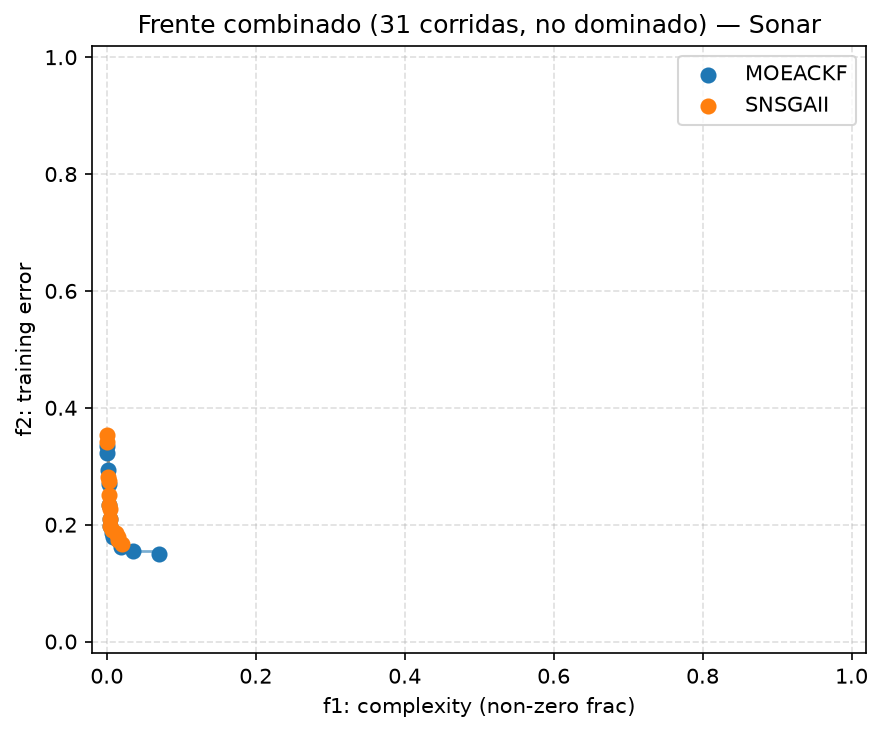
\includegraphics[width=0.75\textwidth]{fronts/ds4_combined_front.png}
\caption{Frente combinado de MOEACKF vs.\ SNSGAII, dataset 4 (Sonar).}
\label{fig:combined-front-ds4}
\end{figure}

Pese a que ambos frentes combinados tienen el mismo tamaño (Figura~\ref{fig:combined-front-ds4}),
este resultado constituye la evidencia más contundente del estudio de que un algoritmo puede
dominar ``punto a punto'' a otro, y no solo en el resumen agregado de HV.

\textbf{Error por banda de complejidad}, Figura~\ref{fig:complexity-bands-ds4}.

\begin{figure}[htbp]
\centering
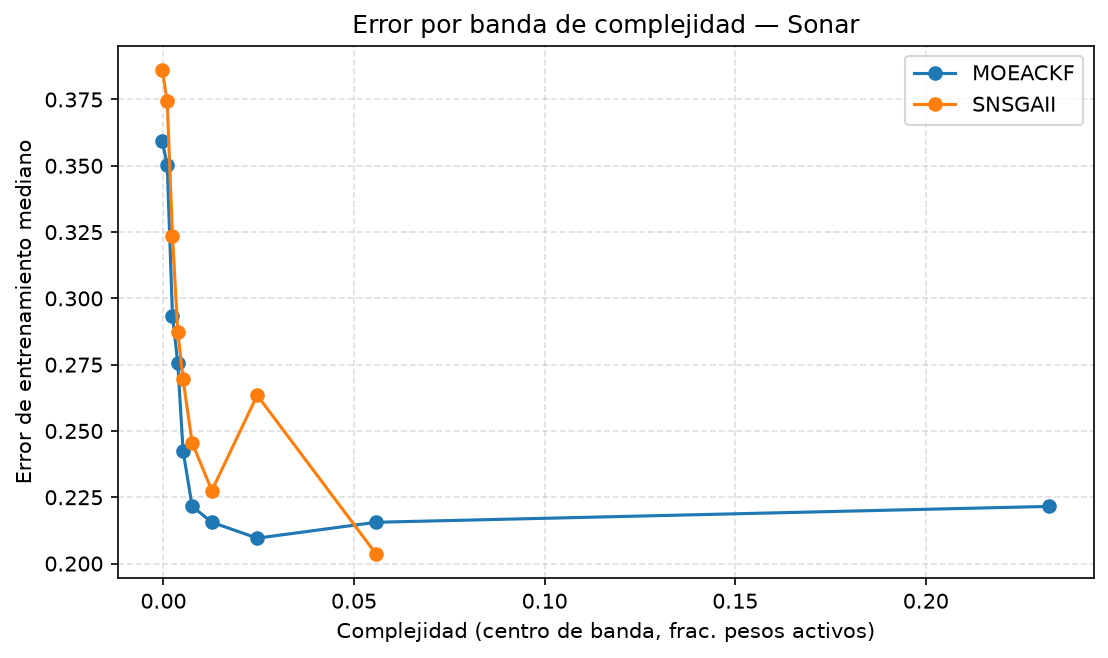
\includegraphics[width=0.75\textwidth]{fronts/ds4_complexity_bands.png}
\caption{Error de entrenamiento mediano por banda de complejidad, dataset 4 (Sonar).}
\label{fig:complexity-bands-ds4}
\end{figure}

MOEACKF presenta un error menor que SNSGAII en casi todo el espectro de complejidad, con SNSGAII
apenas por delante en una banda alta y angosta (de muestra pequeña), y con MOEACKF como el único
que alcanza la banda de mayor complejidad. La ventaja de MOEACKF en Sonar es, entonces, amplia y
no se concentra en una sola región del espacio de complejidad, a diferencia de lo que ocurre con
SNSGAII en los datasets 1 y 3.

\subsubsection{Convergencia}
\label{sec:ds4-convergencia}

\begin{figure}[htbp]
\centering
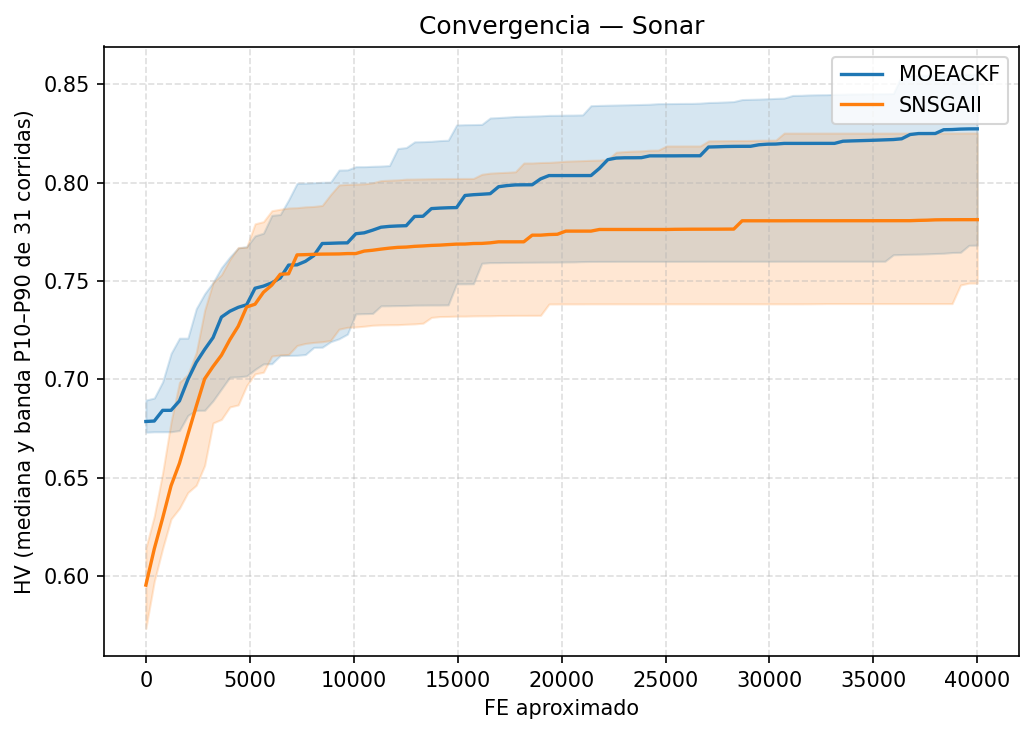
\includegraphics[width=0.75\textwidth]{convergence/ds4_convergence.png}
\caption{Curva de convergencia, dataset 4 (Sonar).}
\label{fig:convergence-ds4}
\end{figure}

Según la Figura~\ref{fig:convergence-ds4}, MOEACKF se mantiene por encima de SNSGAII durante todo
el presupuesto y todavía sigue subiendo lentamente cerca de $\text{FE}=40000$, sin llegar a
aplanarse del todo, mientras que SNSGAII se estabiliza antes ($\text{FE}\approx20000$--$25000$)
en un nivel claramente inferior.

\textbf{Velocidad de convergencia} (FE hasta 95\% del HV final), Tabla~\ref{tab:convergence-speed-ds4}.

\begin{table}[htbp]
\centering
\small
\caption{FE aproximado hasta alcanzar el 95\% del HV final de cada corrida, dataset 4.}
\label{tab:convergence-speed-ds4}
\begin{tabular}{@{}lccc@{}}
\toprule
\textbf{Grupo} & \textbf{Mediana [IQR]} & \textbf{$p$ (Wilcoxon)} &
  \Atwelve \\
\midrule
MOEACKF & $13626.4\ [10622.7,\,18901.1]$ & --- & --- \\
SNSGAII & $5614.0\ [4110.3,\,6416.0]$ & $9.16\times10^{-6}$* & 0.903 \\
\bottomrule
\end{tabular}
\end{table}

La diferencia es significativa tras corrección ($p=4.58\times10^{-5}$), y aquí se invierte la
relación entre velocidad y calidad observada en el dataset 3: el algoritmo con \textbf{menor} HV
final (SNSGAII) converge más rápido a su propio techo, mientras que MOEACKF, con mayor HV final,
tarda $\sim2.4\times$ más (mediana FE $13626$ vs.\ $5614$) en llegar al 95\% del suyo y, según la
curva, todavía no se estabiliza del todo al final del presupuesto. Esto sugiere que MOEACKF
podría beneficiarse de un presupuesto de FE aún mayor en problemas de alta dimensionalidad como
Sonar, lo que constituye un experimento natural para trabajo futuro.

\subsubsection{Plataforma: SNN (C++) vs.\ ANN (MATLAB original)}
\label{sec:ds4-plataforma}

\begin{table}[htbp]
\centering
\small
\caption{MOEACKF: SNN vs.\ ANN (MATLAB), dataset 4.}
\label{tab:platform-moeackf-ds4}
\begin{tabular}{@{}lp{3.2cm}p{3.2cm}cc@{}}
\toprule
\textbf{Indicador} & \textbf{MOEACKF: SNN} & \textbf{MOEACKF: ANN-MATLAB} &
  \textbf{$p$ (Mann-Whitney)} & \Atwelve \\
\midrule
HV & mediana $0.8274\ [0.8141,\,0.8432]$ & mediana $0.8740\ [0.8659,\,0.8849]$ &
  $5.89\times10^{-11}$* & 0.016 \\
Complejidad & mediana $0.0429\ [0.0208,\,0.0847]$ & mediana $0.0097\ [0.0063,\,0.0151]$ &
  $2.40\times10^{-6}$* & 0.849 \\
Accuracy & mediana $0.8204\ [0.8024,\,0.8323]$ & mediana $0.8623\ [0.8533,\,0.8742]$ &
  $4.93\times10^{-10}$* & 0.041 \\
\bottomrule
\end{tabular}

\bigskip
\centering
\caption{SNSGAII: SNN vs.\ ANN (MATLAB), dataset 4.}
\label{tab:platform-snsgaii-ds4}
\begin{tabular}{@{}lp{3.2cm}p{3.2cm}cc@{}}
\toprule
\textbf{Indicador} & \textbf{SNSGAII: SNN} & \textbf{SNSGAII: ANN-MATLAB} &
  \textbf{$p$ (Mann-Whitney)} & \Atwelve \\
\midrule
HV & mediana $0.7812\ [0.7601,\,0.8059]$ & mediana $0.9143\ [0.8994,\,0.9158]$ &
  $1.40\times10^{-11}$* & 0.000 \\
Complejidad & mediana $0.0159\ [0.0077,\,0.0270]$ & mediana $0.1503\ [0.0254,\,0.9942]$ &
  $5.74\times10^{-7}$* & 0.132 \\
Accuracy & mediana $0.7605\ [0.7365,\,0.7874]$ & mediana $0.9102\ [0.9042,\,0.9281]$ &
  $1.32\times10^{-11}$* & 0.000 \\
\bottomrule
\end{tabular}
\end{table}

Todas las comparaciones son significativas tras corrección (Tablas~\ref{tab:platform-moeackf-ds4}
y \ref{tab:platform-snsgaii-ds4}). Para SNSGAII, la brecha ANN-SNN de HV ($0.909$ vs.\ $0.781$,
$\sim0.13$) y de accuracy ($0.915$ vs.\ $0.760$, $\sim0.155$) es la más grande de los cuatro
datasets, lo que sugiere que la alta dimensionalidad de Sonar penaliza más al sustrato SNN que al
ANN, al menos para este algoritmo. La complejidad de MOEACKF constituye, además, la
\textbf{única reversión} de las ocho combinaciones plataforma$\times$algoritmo del estudio: aquí
la red SNN de mejor accuracy ($0.079$) es más densa que la ANN ($0.014$), mientras que en el
resto de los casos con una brecha clara de complejidad es la ANN la más densa. Vale la pena
señalar esta excepción explícitamente en la tesis, en lugar de asumirla como parte del patrón
general.

\subsubsection{Bootstrap vs.\ evaluación completa}
\label{sec:ds4-bootstrap}

\begin{sidewaystable}
\centering
\small
\caption{HV con evaluación normal vs.\ bootstrap, y multiplicador de tiempo de cómputo, dataset 4.}
\label{tab:bootstrap-ds4}
\begin{tabular}{@{}lp{3.4cm}p{3.4cm}ccp{3.6cm}@{}}
\toprule
\textbf{Algoritmo} & \textbf{Normal} & \textbf{Bootstrap} & \textbf{$p$ (Wilcoxon)} & \Atwelve &
  \textbf{Tiempo mediano ($\times$)} \\
\midrule
MOEACKF & mediana $0.8274\ [0.8141,\,0.8432]$ & mediana $0.8356\ [0.8157,\,0.8424]$ &
  $0.2241$ & 0.484 & $1832\text{ s} \rightarrow 9202\text{ s}$ ($\times5.0$) \\
SNSGAII & mediana $0.7812\ [0.7601,\,0.8059]$ & mediana $0.8066\ [0.7753,\,0.8272]$ &
  $0.0132$* & 0.290 & $1730\text{ s} \rightarrow 11884\text{ s}$ ($\times6.9$) \\
\bottomrule
\end{tabular}
\end{sidewaystable}

Este dataset muestra un patrón inverso al del dataset 3 (Tabla~\ref{tab:bootstrap-ds4}): aquí el
bootstrap ayuda significativamente a SNSGAII (tras corrección, $p=0.0264$), pero no muestra
efecto en MOEACKF ($p=0.224$, $\Atwelve=0.484$, prácticamente indistinguible del azar). Al
comparar los datasets 3 y 4 queda claro que el beneficio del bootstrap depende de la combinación
específica de dataset y algoritmo, y no de una regla simple del tipo ``siempre ayuda'' o ``ayuda
siempre al mismo algoritmo''; esto se documenta como pregunta abierta en las limitaciones
(\S\ref{sec:limitaciones}).

\subsubsection{Tiempo de cómputo}
\label{sec:ds4-tiempo}

\begin{table}[htbp]
\centering
\small
\caption{Tiempo de ejecución (\texttt{time\_s}), dataset 4, $N=15$ corridas pareadas.}
\label{tab:time-ds4}
\begin{tabular}{@{}lccc@{}}
\toprule
\textbf{Grupo} & \textbf{Mediana [IQR]} & \textbf{$p$ (Wilcoxon)} &
  \Atwelve \\
\midrule
MOEACKF & $715.1\ [525.9,\,865.2]$ s & --- & --- \\
SNSGAII & $295.5\ [294.0,\,298.2]$ s & $6.10\times10^{-5}$* & 1.000 \\
\bottomrule
\end{tabular}
\end{table}

Según la Tabla~\ref{tab:time-ds4}, esta es la diferencia significativa más extrema del estudio:
$\Atwelve=1.000$, con SNSGAII más rápido en las 15 corridas pareadas, sin una sola excepción.
MOEACKF resulta aquí $\sim2.4\times$ más lento ($715$ vs.\ $296$ s medianos) y con una
variabilidad de tiempo mucho mayor (DE$=259.5$s, muy por encima del resto de los datasets), lo
cual es consistente con que su mecanismo de fusión de conocimiento entre escalas (SVD, análisis
de dispersión) escala peor con la dimensionalidad (60 features) que los operadores más simples de
SNSGAII.

\subsection{Síntesis entre datasets (descriptiva, no un test adicional)}
\label{sec:sintesis}

En cumplimiento del requisito de no combinar datasets en una misma prueba estadística, esta
sección tiene un carácter puramente \textbf{descriptivo}, en el espíritu de Demšar (2006).

\textbf{HV principal}: SNSGAII gana en 2 de los 4 datasets (ds1, ds3), MOEACKF en 1 (ds4), y en 1
no hay diferencia significativa (ds2), sin cambios respecto al análisis original. Se mantiene la
hipótesis, no probada estadísticamente con solo cuatro puntos, de que SNSGAII rinde mejor en
datasets de menor dimensionalidad (14 y 24 features) y MOEACKF en el de mayor dimensionalidad (60
features), mientras que en el de dimensionalidad intermedia (18 features) no hay diferencia. Los
ángulos de comparación incorporados en este análisis refuerzan esta lectura con más matices:

\begin{itemize}
  \item \textbf{Frentes}: en ds1 y ds3, los datasets que gana SNSGAII, su solución de mejor
        accuracy es más densa y más precisa que la de MOEACKF; en ds4, que gana MOEACKF, el
        patrón se repite pero con los roles invertidos, ya que es MOEACKF quien gana en densidad
        y precisión a la vez. El C-metric del frente combinado es más parejo en ds2/ds3
        ($0.50/0.50$, $0.31/0.33$) y muy asimétrico en ds4 ($0.86/0.14$ a favor de MOEACKF), de
        modo que el dataset con la victoria de HV más contundente es también el de dominancia
        punto a punto más contundente.
  \item \textbf{Convergencia}: en los tres datasets donde existe una diferencia clara de HV (ds1,
        ds3, ds4), el algoritmo que \textbf{pierde} en HV final es sistemáticamente el que
        converge más rápido a su propio techo ($\Atwelve$ de velocidad $\approx0.00$ para
        MOEACKF en ds1/ds3, $\approx0.90$ para MOEACKF en ds4, siempre a favor del algoritmo de
        menor HV). Un plateau rápido en un techo bajo frente a un ascenso lento hacia un techo
        alto parece ser, entonces, un trade-off recurrente en este estudio, y no el ruido de una
        sola corrida.
  \item \textbf{Tiempo}: SNSGAII es más rápido en los cuatro datasets, pero la brecha crece
        marcadamente con la dimensionalidad, de $\sim6$--$10\%$ en ds1--ds3 (14--24 features) a
        $\sim2.4\times$ en ds4 (60 features, $\Atwelve=1.000$). Esto es consistente con que
        MOEACKF consume más FE por generación que SNSGAII (ver \S\ref{sec:convergencia}), y con
        que ese costo adicional escala con el tamaño del problema.
  \item \textbf{Plataforma}: es el hallazgo más uniforme de todo el análisis. La ANN original
        (MATLAB) supera a la SNN en HV y accuracy en las \textbf{8 de 8} combinaciones
        dataset$\times$algoritmo, siempre de forma significativa tras corrección. La brecha de
        accuracy es más pequeña en ds1 ($\sim0.02$) y más grande en ds4 para SNSGAII
        ($\sim0.155$). La brecha de complejidad entre ANN y SNN para SNSGAII (extrema en ds2/ds3,
        moderada en ds1/ds4) es sistemáticamente mayor que la de MOEACKF (siempre moderada), un
        patrón dependiente del algoritmo que se repite entre datasets y que podría merecer
        investigación aparte.
  \item \textbf{Bootstrap}: mejora el HV de forma clara y consistente en ds1 y ds2, con efecto
        grande en ambos algoritmos, pero produce resultados mixtos en ds3 (solo ayuda a MOEACKF)
        y en ds4 (solo ayuda a SNSGAII). No existe, entonces, una regla simple, y el costo de
        tiempo ($\times4.8$ a $\times15.1$) es siempre sustancial, independientemente de si el HV
        mejora o no.
\end{itemize}

También se mantiene la observación original: en 3 de los 4 datasets (ds1, ds2, ds3) MOEACKF
muestra menor varianza entre corridas que SNSGAII en HV, incluso cuando pierde en mediana, es
decir, MOEACKF tiende a ser más consistente y predecible. Si el criterio de la tesis valora la
reproducibilidad además del desempeño puntual, esta observación sigue siendo relevante más allá
de qué algoritmo ``gana'' cada test.

\subsection{Limitaciones de este análisis}
\label{sec:limitaciones}

\begin{itemize}
  \item \textbf{Accuracy de test}: se trata de una limitación \textbf{estructural}, no de un dato
        pendiente de calcular. El 100\% de las corridas archivadas en \texttt{normal\_results} y
        \texttt{bootstrap\_results} usan una arquitectura de 2 salidas (WTA), y el código solo
        exporta \texttt{*\_spikes.csv} (necesario para reconstruir la accuracy de test) cuando
        \texttt{nOutputs == 1}. Con los datos actuales no es posible medir la generalización de
        forma directa; el análisis de frentes (\S\ref{sec:ds1-fronts}--\S\ref{sec:ds4-fronts})
        funciona como el sustituto disponible, al examinar la relación complejidad-error de todo
        el frente en lugar de un valor puntual de accuracy de test.
  \item \textbf{Datasets 5 y 6 (Iris, Wine) no tienen resultados corridos} en ninguna de las
        cuatro fuentes, por lo que las conclusiones de este documento cubren únicamente Statlog
        Australian, Climate, German y Sonar.
  \item \textbf{Tiempo de cómputo}: \texttt{normal\_results} y \texttt{bootstrap\_results} siguen
        sin permitir una comparación válida de \texttt{time\_s}, debido al paralelismo y los
        hilos no controlados entre tandas de ejecución. Solo \texttt{time\_experiments}
        (\S\ref{sec:ds1-tiempo}--\S\ref{sec:ds4-tiempo}) permite una comparación de tiempo válida,
        pero se ejecutó con hiperparámetros compartidos, no afinados por algoritmo; por ello, sus
        conclusiones de tiempo no deben mezclarse con las conclusiones de calidad (HV) del resto
        del análisis, que sí emplea hiperparámetros afinados.
  \item \textbf{Comparación de plataforma (SNN vs.\ ANN)}: MATLAB/PlatEMO original y el port en
        C++ difieren en más que el modelo de neurona, ya que también difieren en la
        implementación y en el generador de números aleatorios; al no existir columna de seed en
        los datos de MATLAB, no hay forma de aislar esa diferencia. Por ello, los resultados de
        \S\ref{sec:ds1-plataforma}--\S\ref{sec:ds4-plataforma} deben leerse como evidencia
        direccional (la ANN supera consistentemente a la SNN), y no como una atribución causal
        limpia al hecho de ser spiking.
  \item \textbf{Bootstrap}: el régimen de evaluación modifica el ruido de la señal de fitness, y
        su efecto sobre el HV final resulta mixto entre dataset y algoritmo
        (\S\ref{sec:ds3-bootstrap}, \S\ref{sec:ds4-bootstrap}), sin que se haya identificado un
        patrón simple. Queda como pregunta abierta si existe alguna interacción entre el
        remuestreo y los mecanismos específicos de cada algoritmo (p.\,ej.\ el filtro de Kalman
        de MOEACKF).
  \item \textbf{C-metric sobre frentes combinados pequeños}: los frentes combinados de 31
        corridas quedan reducidos a 4--14 puntos tras deduplicar y filtrar los no dominados, de
        modo que la resolución de la métrica de cobertura es limitada en conjuntos tan pequeños.
        Por ello, se reporta como una magnitud aproximada y no como una proporción de alta
        precisión.
  \item \textbf{FE aproximado en convergencia}: \texttt{convergence.csv} no registra el FE por
        fila, sino solo la \texttt{generation}, que no es comparable entre algoritmos porque
        MOEACKF consume más FE por generación que SNSGAII. En consecuencia, el eje FE de las
        curvas y de los umbrales de velocidad
        (\S\ref{sec:ds1-convergencia}--\S\ref{sec:ds4-convergencia}) es una aproximación por
        interpolación lineal dentro de cada corrida, y no un valor exacto por fila.
\end{itemize}
